\documentclass{article}

% Language setting
\usepackage[english]{babel}

% Set page size and margins
\usepackage[letterpaper,top=2cm,bottom=2cm,left=3cm,right=3cm,marginparwidth=1.75cm]{geometry}

% Useful packages
\usepackage{amsmath}
\usepackage{graphicx}
\usepackage[colorlinks=true, allcolors=blue]{hyperref}
\usepackage{listings}
\lstset{
    language=C,
    extendedchars=true,
    basicstyle=\tt\footnotesize,
    numbers=left, 
    numberstyle=\tiny, 
    stepnumber=2, 
    numbersep=5pt,
    lineskip=-2pt
}

\title{Programmation Parall\'ele}
\author{Lucas Marques, Matis Duval}

\begin{document}
\maketitle

\begin{abstract}
Rapport Projet: Le jeu de la vie
\end{abstract}

\section{Introduction}
Ce projet s'inscrit dans le cadre de l'étude de la programmation parallèle appliquée à la simulation du \href{https://en.wikipedia.org/wiki/Conway%27s_Game_of_Life}{Jeu de la Vie} de Conway. L'objectif est d'optimiser l'exécution du programme en exploitant les capacités parallèles des architectures modernes.

\section{Utilisation de EasyPaP}
EasyPaP est un framework utilisé pour exécuter et analyser des simulations parallèles. Il nous permet d'observer l'impact de différentes stratégies de parallélisation sur la performance et d'obtenir des métriques précises sur le comportement du programme. Nous l'avons utilisé pour générer les traces et mesurer le temps d'exécution des différentes optimisations mises en place.

\section{Premier Jalon}

\textbf{Parall\'elisation de base (salle 008) [Vendredi 28 février]}

On ajoute les fonctions demandées:

\begin{lstlisting}
unsigned life_compute_ompfor (unsigned nb_iter)
{
  unsigned res = 0;

  for (unsigned it = 1; it <= nb_iter; it++) {
    unsigned change = 0;

    #pragma omp parallel for schedule(dynamic) collapse(2)
    for (int y = 0; y < DIM; y += TILE_H)
      for (int x = 0; x < DIM; x += TILE_W) {
        #pragma omp atomic
        change |= life_do_tile_default (x, y, TILE_W, TILE_H);
      }

    #pragma omp single
    swap_tables ();

    if (!change) { // we stop if all cells are stable
      res = it;
      break;
    }
  }

  return res;
}
\end{lstlisting}

\section{Modifications et Optimisations du Code}

Nous avons apporté plusieurs modifications au code afin d'améliorer ses performances. Voici quelques versions mises à jour avec leurs justifications :

\subsection{Optimisation avec OpenMP Task}

\begin{lstlisting}
unsigned life_compute_omptaskloop(unsigned nb_iter)
{
  int tuile[TILE_H][TILE_W + 1] __attribute__ ((unused));
  for (unsigned it = 1; it <= nb_iter; it++) {
    unsigned change = 0;

#pragma omp master
    for (int y = 0; y < DIM; y += TILE_H)
      for (int x = 0; x < DIM; x += TILE_W)
        #pragma omp task firstprivate(y, x) depend(out: tuile[y][x]) depend(in: tuile[y-1][x], tuile[y][x-1])
        change |= life_do_tile_default (x, y, TILE_W, TILE_H);

    swap_tables ();
  }
  return 0;
}
\end{lstlisting}

Cette optimisation remplace la parallélisation par boucle avec `omp task`, permettant une meilleure gestion des dépendances et une charge mieux équilibrée.

\section{Expérimentations et Résultats}

Nous allons tester différentes configurations de simulation pour analyser leurs impacts sur les performances.

\subsection{Variation de la Taille de Simulation}
Nous testons les tailles suivantes: 256, 512, 1024, 4096, 8192. L'objectif est d'observer comment la taille de la grille influence l'efficacité du parallélisme.

\begin{figure}[h]
    \centering
    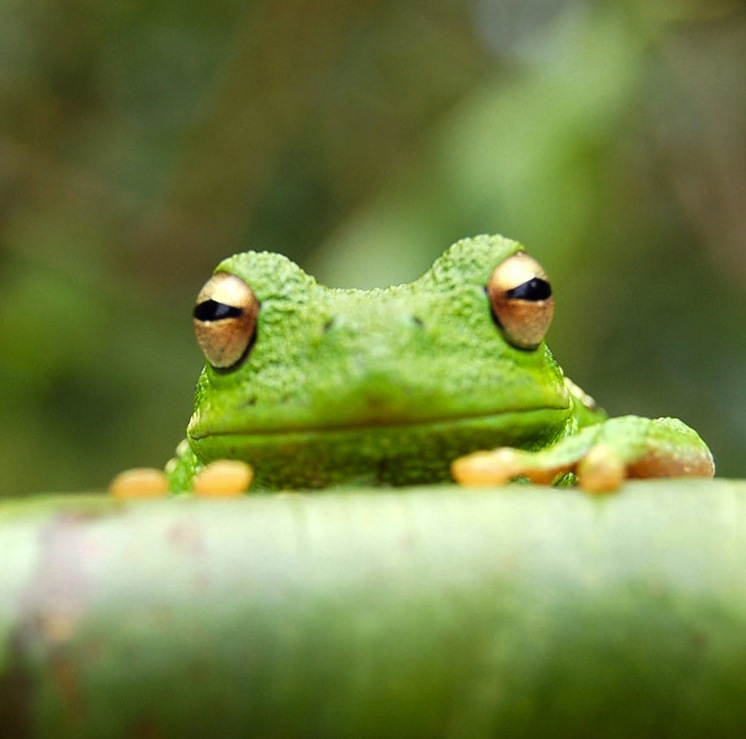
\includegraphics[width=0.8\textwidth]{frog.jpg}  % Remplacer par le vrai graphique
    \caption{Temps d'exécution en fonction de la taille de la simulation}
    \label{fig:taille_simulation}
\end{figure}

\subsection{Effet du Nombre de Threads}
Nous analysons l'impact du nombre de threads sur la performance, en testant entre 0 et 12 threads.

\begin{figure}[h]
    \centering
    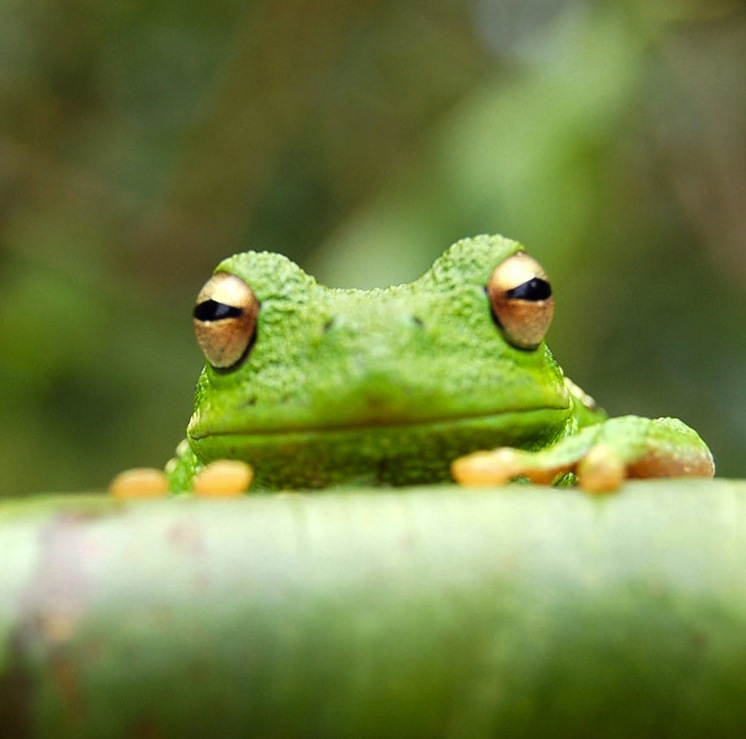
\includegraphics[width=0.8\textwidth]{frog.jpg}  % Remplacer par le vrai graphique
    \caption{Impact du nombre de threads sur la vitesse d'exécution}
    \label{fig:nb_threads}
\end{figure}

\subsection{Effet de la Taille des Tuiles}
Nous testons différentes tailles de tuiles et leur interaction avec le nombre de threads.

\begin{figure}[h]
    \centering
    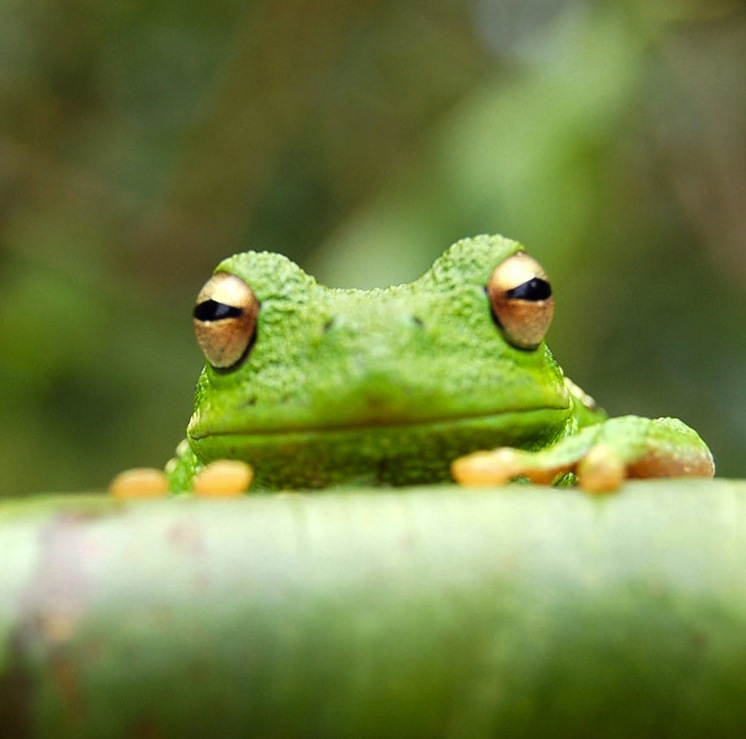
\includegraphics[width=0.8\textwidth]{frog.jpg}  % Remplacer par le vrai graphique
    \caption{Temps d'exécution selon la taille des tuiles et le nombre de threads}
    \label{fig:taille_tuiles}
\end{figure}

\subsection{Comparaison des Distributions Statiques et Dynamiques}
Nous analysons l'impact de la distribution du travail (statique vs dynamique) sur les performances.

\begin{figure}[h]
    \centering
    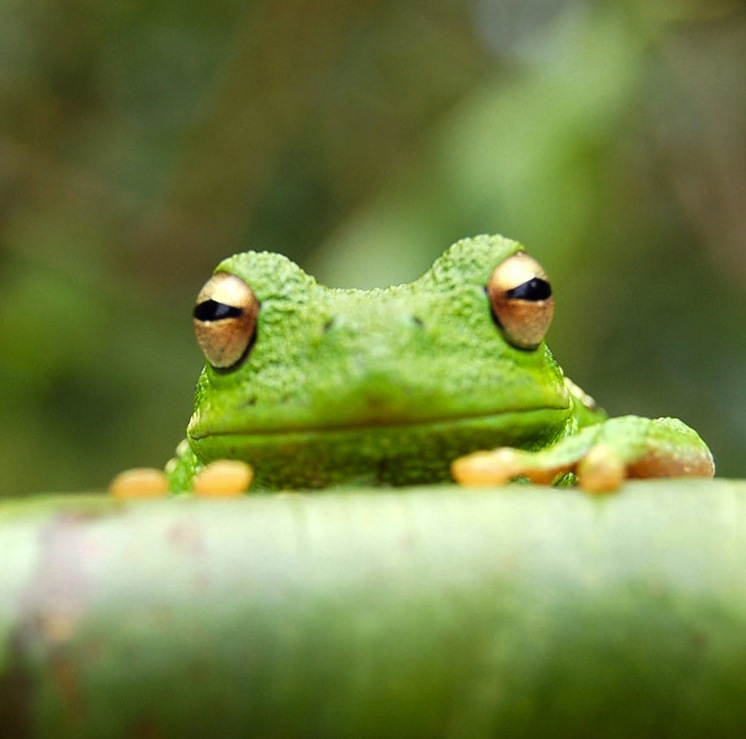
\includegraphics[width=0.8\textwidth]{frog.jpg}  % Remplacer par le vrai graphique
    \caption{Comparaison des stratégies de distribution de charge}
    \label{fig:distribution_charge}
\end{figure}

\subsection{Comparaison GCC vs Clang}
Nous testons l'impact du compilateur sur les performances.

\begin{figure}[h]
    \centering
    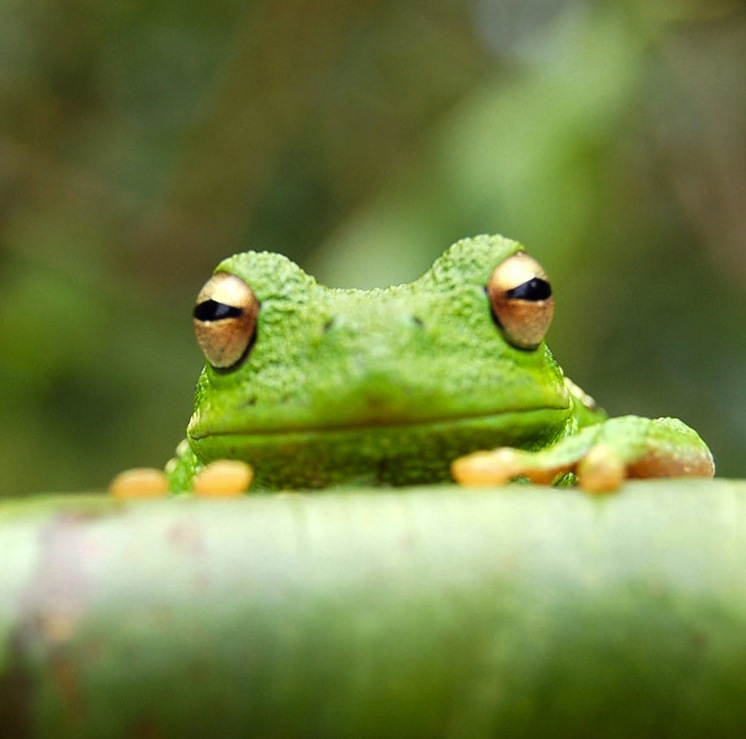
\includegraphics[width=0.8\textwidth]{frog.jpg}  % Remplacer par le vrai graphique
    \caption{Comparaison des performances entre GCC et Clang}
    \label{fig:gcc_vs_clang}
\end{figure}

\section{Analyse des Résultats}
Nous expliquerons ici les observations faites à partir des graphes ci-dessus, en nous basant sur des éléments comme la mémoire cache, la contention, l'équilibrage de charge, etc.

\end{document}
